\documentclass[10pt,final,journal,a4paper,oneside,twocolumn]{IEEEtran}

\usepackage[english,german]{babel}
\usepackage[utf8]{inputenc}
\usepackage[T1]{fontenc}
\usepackage{cite}
\usepackage{amsmath,amssymb,amsfonts}
\usepackage{algorithmic}
\usepackage{graphicx}
\usepackage{textcomp}
\usepackage{xcolor}
\usepackage[absolute]{textpos}
\usepackage{hyperref}
\usepackage{float}
\DeclareMathOperator*{\argmax}{argmax} % thin space, limits underneath in displays

\usepackage{eurosym}
\usepackage{listings}
\usepackage{color}
\renewcommand{\lstlistingname}{Code}

\usepackage{listings}
\usepackage{xcolor}

\usepackage{tabularx}

\colorlet{punct}{red!60!black}
\definecolor{background}{HTML}{EEEEEE}
\definecolor{delim}{RGB}{20,105,176}
\colorlet{numb}{magenta!60!black}

\lstdefinelanguage{json}{
	belowcaptionskip=1\baselineskip,
	captionpos=b,
	lineskip=4pt,
	frame=none,
	xleftmargin=0pt, 
	xrightmargin=0pt,
	aboveskip=10pt,
	belowskip=10pt,
	showstringspaces=false,
	basicstyle=\footnotesize\ttfamily,
	keywordstyle=\color{darkblue},
	commentstyle=\itshape\color{mygreen},
	identifierstyle=\color{black},
	backgroundcolor=\color{myrandom}, 
	stringstyle=\color{darkblue},
	morekeywords={intent, entities}
}
\definecolor{mygreen}{rgb}{0,0.4,0}
\definecolor{myred}{rgb}{0.8,0.16,0}
\definecolor{myrandom}{RGB}{255, 248, 246}
\definecolor{darkblue}{rgb}{0.0,0.0,0.6}
\lstset{
	belowcaptionskip=1\baselineskip,
	captionpos=b,
	lineskip=4pt,
	frame=none,
	xleftmargin=0pt, 
	xrightmargin=0pt,
	aboveskip=10pt,
	belowskip=10pt,
	language=XML,
	showstringspaces=false,
	basicstyle=\footnotesize\ttfamily,
	keywordstyle=\color{darkblue},
	commentstyle=\itshape\color{mygreen},
	identifierstyle=\color{black},
	backgroundcolor=\color{myrandom}, 
	stringstyle=\color{mygreen},
	morekeywords={category, pattern, template, topic, srai, aiml}
}
\def\BibTeX{{\rm B\kern-.05em{\sc i\kern-.025em b}\kern-.08em
    T\kern-.1667em\lower.7ex\hbox{E}\kern-.125emX}}

\renewcommand\footnoterule{\kern-3pt \hrule width 3.5in \kern 2.6pt}


\renewcommand\IEEEkeywordsname{Keywords}

\begin{document}

\selectlanguage{english}
\title{
	Chatbots: Basics and Frameworks\\
	\small Advanced Topics in AI - WS19/20
}

\author{
\IEEEauthorblockN{{\large Fabio Aubele}}\\
\IEEEauthorblockA{Faculty of Computer Science\\
University of Applied Sciences\\
Augsburg, Germany\\
fabio.aubele@hs-augsburg.de \\}
\and
\IEEEauthorblockN{{\large Joshua Hörmann}}\\
\IEEEauthorblockA{Faculty of Computer Science\\
University of Applied Sciences\\
Augsburg, Germany\\
joshua.hoermann1@hs-augsburg.de}
}
\maketitle

\begin{abstract}
This paper focus on teaching the basics of Chatbots and presenting three frameworks based on this. First the difference between the main two types of Chatbots are worked out. Then the general work methods of a bot are defined and explained in consideration of the two different types of Chatbots. For every work method there are two concrete examples, which show, how it is feasible to realise them. Afterwards, three frameworks are presented, the focus lies on showing the concept, general functioning and key features of each framework, so it is possible to assess, for which use case the different frameworks are optimal. Thereupon the different deployment options are presented and evaluated. Finally the frameworks are compared and pros and cons are listed.
\end{abstract}

\begin{IEEEkeywords}
Chatbot, Conversational AI, Chatbot Frameworks, Rule-based, Artificial Intelligence, AIML, Rasa, Dialogflow
\end{IEEEkeywords}

\section{Introduction (both)}
It is common knowledge, that almost any gadget, which uses the technology 'Artificial Intelligence' (AI), gets a lot of attention in today's time. The spectrum of AI includes every process, where a machine demonstrates intelligence. One of the earliest idea, which fascinated humans, was the possibility, to communicate with a computer. Already in 1966 one of the first Chatbots ELIZA was published \cite{b1}, which should simulate a psychotherapist. The creator of the program Joseph Weizenbaum never claimed, that ELIZA is intelligent. The only idea behind it was, to show the public the superficiality of communication between humans and machine. In order to achieve this, the key method of the application was, to recognize certain phrases or words and then formulating an answer with a pre-programmed response \cite{b1}. This technique is also known as pattern matching. With this approach ELIZA also achieved, that some people attributed human-like feelings, while they were communicating with the bot.\\
Obviously technology evolved really far. Nowadays a lot of companies are using Chatbots, to communicate with their clients. Often Chatbots run on platforms like Facebook, WhatsApp or Skype. Each platform has its own salient features, which determine the possible ways, in which the Chatbot can interact with the user. On Twitter businesses have now the possibility, to create automated welcome messages, present customers with a range of topics and direct their query, without involving a human at all \cite{b2}.
\begin{figure}[htbp]
	\centerline{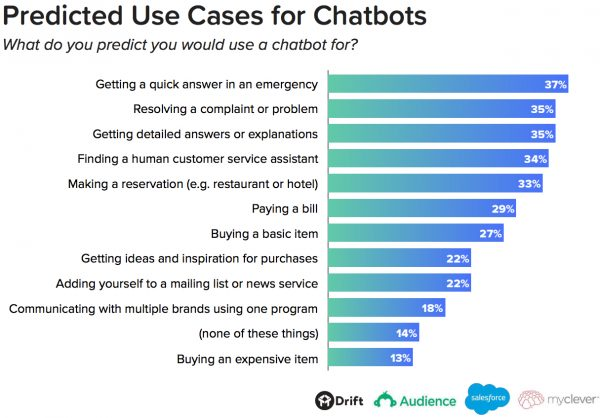
\includegraphics[width=1\linewidth]{pictures/Statistic.jpg}}
	\caption{Predicted use cases for Chatbots\cite{b3}.}
	\label{statistic}
\end{figure}
\\
In figure \ref{statistic} a statistic is seen, that shows the predicted use cases for Chatbots. A brief description got provided in the survey, which explained how Chatbots work. Then the participants got asked: 'What do you predict you would use a Chatbot for?'. Almost all answers are related to problems, that usually get solved by a customer support. Only simple tasks like 'paying a bill', 'making a reservation' and 'buying a basic item' are the exceptions. This makes a lot of sense, since the most frequent field for bot services are websites or programs, where they are used for contacting the customer, to solve smaller problems or forward bigger problems, help them navigate through the website or give out general informations. Therefore, Chatbots are a feasible customer service channel. And this is just the beginning, in the future these bot services will be able to handle even more complex problems and tasks, as technology advances and data quantities grow.\\
\\
Since the demand for Chatbots is so high, there are also a lot of systems and frameworks on the market. All those are build differently and used for different purposes. For someone who wants to program a Chatbot for a specific use-case, it can be really hard to find the best framework, since the variety on the market is so wide.\\
Therefore, the purpose of this paper is, to present and evaluate the most popular frameworks. Additionally, it is indicated, for what areas of application the frameworks can be used, so it is easy to decide, if the framework is suitable for certain use cases. In order to have a bigger context and understanding for this subject, the foundations and different types of Chatbots are showcased at the beginning. Furthermore, the different types of deployment are discussed. \\
This paper starts with working out the basics, therefore the terms Conversational AI and Chatbot are defined. After that, the two main types of Chatbots are explained and their advantages/disadvantages are named. Then the general work methods of a bot are shown, which are Natural Language Processing, Response Generation, Knowledge Base Creation and Dialogue Management. For each part there are two examples given, which show, how it is feasible to realise them in consideration of the two different types of Chatbots. Afterwards the frameworks AIML, Rasa and Google's Dialogflow are presented. For each framework, the concept, general functioning and key features are showcased. Thereafter the different ways of deployment are introduced and evaluated based on various key points. Finally the three frameworks are compared with each other and some pros and cons are mentioned.

\section{Related Works (both)}
For the given topic there are several scientific related works. The paper from M. Dahiya \cite{b3} describes, how it is possible, to design and implement a Chatbot. First she starts, to explain the basic design of a Chatbot. Therefore different terms are defined and important design decisions are outlined. Furthermore, all the necessary steps to implement a Chatbot, are clarified. Also, the author is stressing the characteristics of the shown Chatbot in comparison to other concepts. The paper is missing the opportunity, to present Chatbots, that are using Machine Learning, to understand the user and generate a fitting answer. In addition the paper is not introducing any frameworks, which can help to establish a Chatbot.\\
\\
The next paper presents an overview of ALICE, which is a Chatbot in AIML format \cite{b5}. The authors are starting, with explaining the system architecture from ALICE. Since this is defined through the specifications from AIML, they are showcasing the used syntax and techniques of the given framework. After those general informations the authors are presenting their Java program, which allows, to convert readable text to AIML format. This generated information is then used, to enhance the Chatbot. The AIML generation is done with several text sets like normal conversations, monologues and structural FAQ/QA corpora. At the end the results from the different text sets are compared to each other and a conclusion is drawn. The paper is lacking to introduce the topic Chatbots probably, so there are no informations about the basics or different types of Chatbots. Also, no other frameworks are presented or compared to AIML.\\
\\
In Source \cite{b6} an introduction to design choices, architectures, and algorithms used in Chatbots are given. This paper is structured in two parts. In the first part the author is presenting some historical facts and evaluation criteria for the bots. The second part is describing Chatbot functionalities very detailed. The first functionality is Speech-To-Text-Conversion, where some approaches are described. Then the author presents statistical concepts for natural language processing and the mathematical basics for it. Furthermore, three main parts of a Chatbot are explained: Response Generation, Knowledge Base Creation and Dialogue Management. For all those three parts different approaches are showcased. Additionally, the paper outlines the possibility, to create a Text-to-Speech-System. At the end the author is focusing on a case study of IBM Watson’s Chatbot and is concluding with a discussion about security considerations and different applications. Overall the presented work gives a wide overview over the topic, but does not include a general differentiation between the two different types of Chatbots. Also, not more then just one framework is presented, that can help, to program a Chatbot.

\section{Basics (Fabio Aubele)}
The topic Chatbots can be defined really broad, thus it is necessary, to classify the topic correctly. So this chapter starts with explaining, what 'Conversationl AI' means and how it is related to the term Chatbots. After that the two basic types of Chatbots are presented and their different functions, advantages/disadvantages are shown. 

\subsection{Conversational AI}
A common mistake is, that Conversational AI is set equal to the term Chatbots. Certainly, Conversational AI is a generic term, which includes more then just Chatbots. Generally spoken, Conversational AI is a set of technologies, which is enabling the software, to understand and to naturally enter in conversations with humans, using either spoken or written language \cite{b7}. Also, there are hybrid systems, which use both.\\
Digital assistants like Amazons Alexa or Google Home are technologies, which grew a lot in the last few years and are indispensable for Conversational AI. The main difference between those and regular Chatbots are, that they not only perform conversations but also sophisticated tasks \cite{b7}. For some tasks additional equipment or third party software is needed, but then it is definitely possible, for example, to turn the lights on or off. Other tasks could be, to play music, book a restaurant table or add appointments to a virtual calender. Most of these systems only react to voice commands and they will only answer back through spoken language (Alexa, Google Home). Microsoft's Cortana would be an example for a hybrid system, which response to both written and spoken language.\\
\\
However, Chatbots are mostly used for information gathering and to hold a conversation \cite{b7}. Yet, the distinction between digital assistants and Chatbots is not defined that clearly, because there are also Chatbots, which fulfil easy tasks, like solving a support ticket. In other words digital assistants are the evolution of regular Chatbots.\\
Since this paper focuses on Chatbots, digital assistants will not be discussed here. The main part of the presented technology in this work, is used, for performing conversation and delivering information to the user. Digital assistants use most of these technologies aswell, but also way more complicated methods and approaches.

\subsection{Types of Chatbots}\label{sec::types}
It is necessary to distinguish between two types of Chatbots, that differentiate in the technology they use, to reach their goal. Also, this separation helps, to get a better overview of the presented frameworks in chapter \ref{sec:frameworks}. In this section the functionalities, advantages and disadvantages of both types will be explained.
\\
\subsubsection{Rule-based Chatbots}
The first type answers the questions from the user, based on predefined rules \cite{b8}. This is done via pattern matching, which means, if the question from the user contains certain key words or phrases, a specific pattern gets triggered. Based on the initiated pattern, the bot knows, which answer needs to be displayed. Figure \ref{pattern} is showcasing the process in detail.
\begin{figure}[htbp]
	\centerline{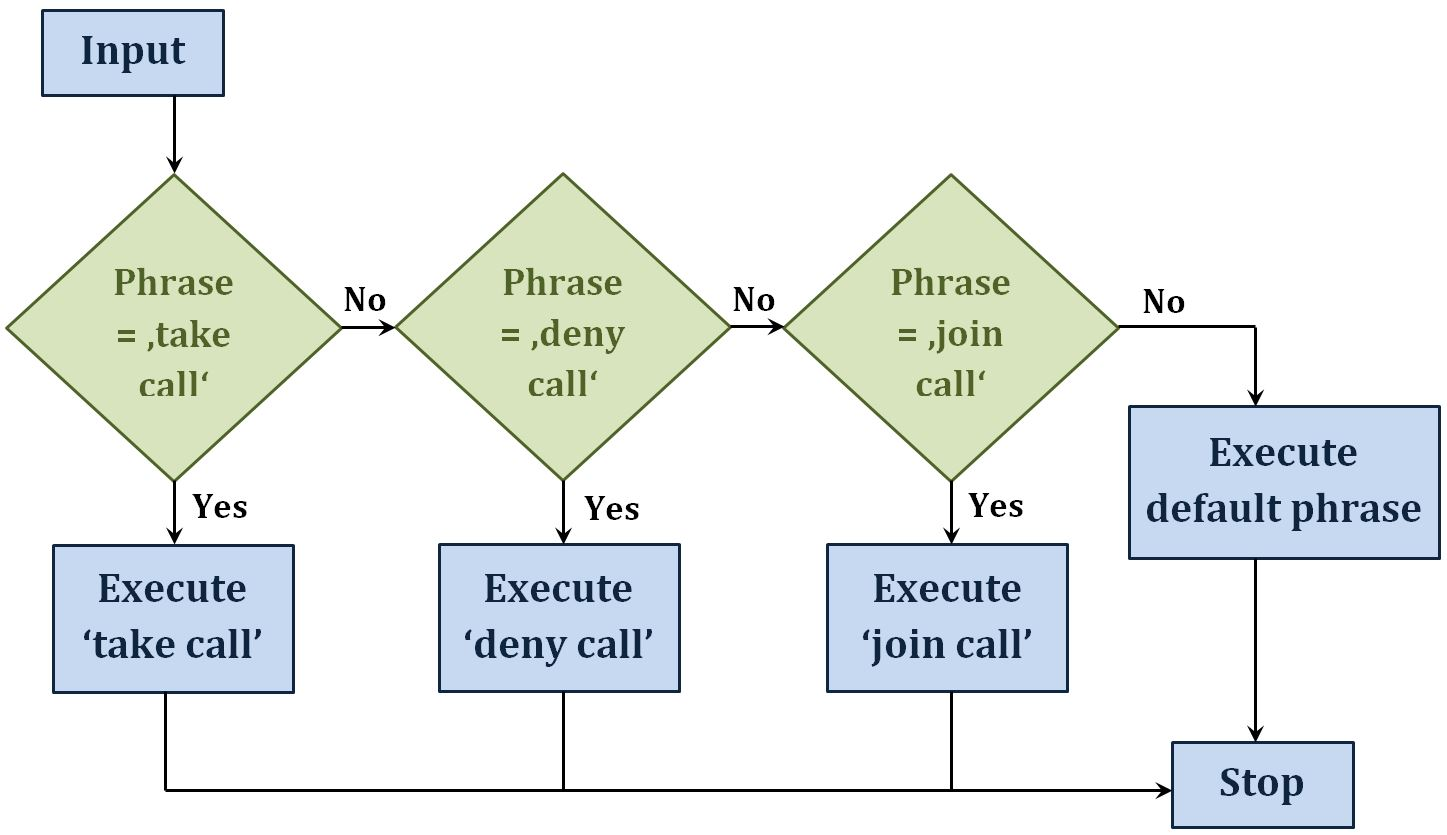
\includegraphics[width=1\linewidth]{pictures/ruleflow.jpg}}
	\caption{Rule-based Chatbot flow (based on \cite{b8}).}
	\label{pattern}
\end{figure}
At the start the given input gets compared to the first pattern, if they correspond with each other, the connected answer to the pattern gets displayed. In the figure \textit{'take call'} is probably not only a response, but also the initiation to start a call. If the input does not fit, the next rule gets checked. When no pattern matches with the input, a default message is issued, which normally expresses, that the Chatbot could not understand the user. Advanced versions of these bots even help the user to find the right questions and phrases, so the user does not trigger the default answer repeatedly. Based on the set of rules, which are defined for the bot, the application case gets specified. Another important part which can influence the set of rules, is the dialogue management, which defines how the bot is handling the conversation with the user. Details for this technique are shown in chapter \ref{sec:dial}.\\
\\
Often bots of this type can only understand simple queries, but fail to manage complex queries \cite{b8}. Also, it is a lot of work, to write patterns for every feasible question, a user can ask, especially when the area of application is complex. However, there are methods that can automate the writing of patterns, even though these approaches are limited and not reliable for every use case. Some frameworks even have a set of downloadable patterns, but most often only for regular conversations. This means that the rules have to be written new in most cases, which automatically creates a limit by nature, since it is not possible to have a endless supply of rules. On the upside it is feasible, to define really precise answers for certain inputs and to create a naive Chatbot quite fast with just a few rules. Additionally, to create this type of bot, no data is needed at the start.
\\
\subsubsection{AI Chatbots}
This type allows, to dissolve the technical border of rule-based Chatbots, which is the reason, that most of today's bots use this approach. In order to achieve this, AI Chatbots are more complicated and use advancements from Machine Learning and Natural Language Processing (NLP), to hold a conversation. Obviously there are many different versions of this type of bot, figure \ref{aiflow} shows a simple version of a flow graph for an AI Chatbot.  
\begin{figure}[htbp]
	\centerline{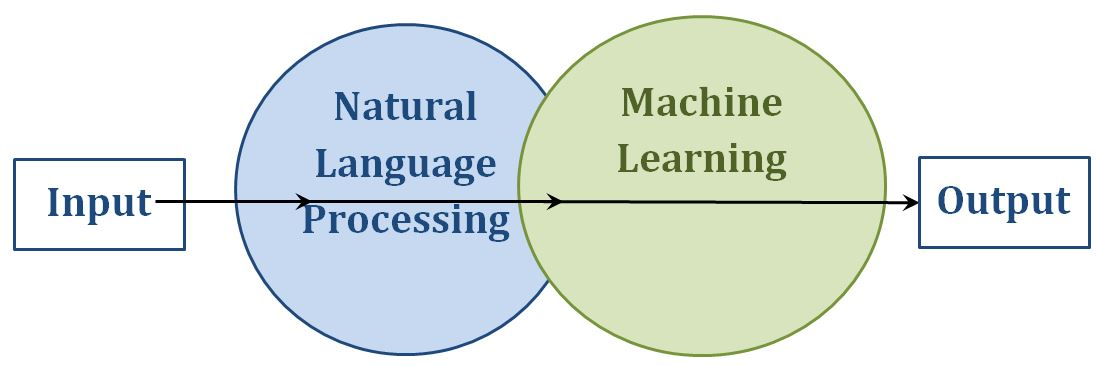
\includegraphics[width=1\linewidth]{pictures/aiflow.jpg}}
	\caption{AI Chatbot flow (based on \cite{b9}).}
	\label{aiflow}
\end{figure}
Mainly, there are two big parts: NLP takes care, to translate the input from the user into a form, the computer can understand and therefore process it further. Then the Machine Learning part generates a response, based on the given information from NLP. It is important to note, that NLP also needs to learn the correct translation with predefined training-data and techniques from Machine Learning. This is why both circles in figure \ref{aiflow} are overlapping. The detailed work methods and architecture are explained in chapter \ref{sec:archi}.\\
\\
AI Chatbots have the advantage, that needed data can be more unstructured and thus do not have to be hand-written. In particular, since the frameworks offer techniques or tools, which helps to generate data easily. Also, this type of bot can get trained with the gathered data, while running and continuously improve, as more data comes in. Additionally, there are no limits, if enough data is available, the bot can be trained for different topics and tasks. On the negative side the selection process for a Machine Learning approach can be quite complex, since they rely on correct configuration and application. Also, the structure of the given training-data needs to be known, to have optimal results.\\

\section{Work Methods (Fabio Aubele)}\label{sec:archi}
This chapter will present an overview of a typical Chatbot system. Therefore, four key work methods will be presented. Not every Chatbot uses all of these methods, it always relies on the given use case and type of the bot. That is why at the start of each section, a classification of the appropriate work method is given. This chapter starts with explaining Natural Language Processing (NLP) and presenting two relevant approaches for it. Then techniques to generate a response to the user, are presented. The next point focuses on the possibility, to create a Knowledge Base for the Chatbot. In the end strategies and tricks are explained, which show, how to manage the dialogue as a bot.

\subsection{Natural Language Processing (NLP)}
One key function of every Chatbot is, to understand, what the user says. In rule-based systems this is done through predefined patterns. An AI bot on the other hand uses NLP for this task. NLP allows, to take the input from the user and transform it into a structure, that the computer understands and uses for further processing \cite{b10}. So without NLP the inputs \textit{'Hello'} and \textit{'Goodbye'} would be text, that the computer can not differentiate. This is quite a complex task, since problems that also hinder the day-to-day communication like wrong spelling, grammatical errors or poor language use in general, need to be identified and interpreted correctly from NLP \cite{b10}. There are multiple approaches, which actually give the typed words some meaning for the machine, two techniques are presented here.
\\
\subsubsection{Intent and Entities}\label{sec:inform}
The primary responsibility of the NLP-engine is, to extract the information from the user in a form, that is understandable for a machine. This first approach works with Intents and Entities. Both Terms need to be defined first:\\
\textbf{Intent:} The central reason a user contacts the Chatbot. This can be a task or a problem, that the user is looking to solve \cite{b10}.\\
\textbf{Entities:} All relevant characteristics or details for the users Intent. This can vary from locations to persons, time, date, etc. \cite{b10}.\\
So for the utterance: \textit{'I want to search a graphic card, that costs 500\euro.'}, the Intent is \textit{'search\_pcpart'} and the Entities are \textit{'graphic card'} and \textit{'500\euro'}. The target of the NLP-engine is, to output the Intent and all Entities for a given sentence and forward this information to the Response Generator (chapter \ref{sec::rg}). For this, it is necessary, to define different types of Intents and Entities. Additionally, many training examples for every type needs to be provided, so it is possible to set-up a Machine Learning model and train it with all the Intents and Entities \cite{b10}. There are different types of appropriate Machine Learning models, in reference \cite[p. 8-19]{b12} a Bayesian and Neural Network approach are presented. These are showcased for a Dialogue Act Recognition system, but they can also be used for this application case \cite{b6}. Now, if the user enters a new utterance, the Machine Learning model and thus the NLP-engine can calculate the similarity between the input and the training examples, hence categorize it as the Intent and Entities with the highest similarity score or as unknown, if it did not exceed a predefined threshold \cite{b10}.\\
\\
In order to achieve the described behaviour, the engine has to understand the meaning of the words, structure from sentences, conjugation and other potential factors, that speech can have. This can be done with the following tasks: \cite{b11}:
\begin{enumerate}
	\item \textbf{Tokenization:} The sentence gets separated into pieces, that represent each of its component parts: words, punctuation marks, numbers, etc.
	\item \textbf{Normalization:} A program processes the text, to find out errors and common spelling mistakes, that might alter the intended meaning.
	\item \textbf{Named Entity Recognition:} The NLP-engine tries to find Entities, based on the given training-data. Therefore, the Entity value in the input is matched with the correct type (\textit{'graphic card'} - part or \textit{'500\euro'} - cost).
	\item \textbf{Intent Classification:} The Chatbot searches for the subjects, verbs, objects, common phrases and nouns in the user’s text, to discover related phrases from the training-data, to find out the Intent.
\end{enumerate}
However, there are many difficulties in this process, especially to tokenize all sentence, is a complex challenge, since the system need to differentiate phrases (\textit{'New York'}) from single words (\textit{'new'}), punctuation at the end of sentences from abbreviations (\textit{'Dr.'}) and more \cite{b6}. Also, there are a lot of linguistic difficulties aswell, like words that actually mean the same (\textit{'right'} as direction or to signalise truth) or sentence structures, where the semantic meaning is not clear. Therefore, a lot of training-data is needed, where all these possibilities are taken into account.
\\
\subsubsection{Dialogue Act Recognition}
One different possibility to extract meaning out of input, is to determine the function of the sentences (question, statement, suggestion, hesitation, command, etc.). For this purpose the sentences need to be labelled with the fitting tags, which expresses the function of it. An example is seen in figure \ref{da}, where every sentence is labelled in the column 'Dialogue Act'.
\begin{figure}[htbp]
	\centerline{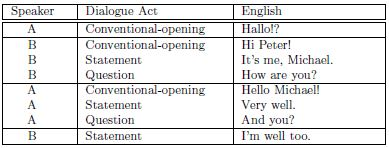
\includegraphics[width=1\linewidth]{pictures/da.jpg}}
	\caption{Example for Dialogue Act Recognition \cite{b12}.}
	\label{da}
\end{figure}
At the beginning all possible tags, need to be defined, which is quite difficult, because the tags need to have three conflicting requirements \cite{b12}:
\begin{itemize}
	\item The tag need to be generic enough, to be useful for different task.
	\item The tag must be specific enough, to encode detailed and exploitable
	characteristics of the target task.
	\item The tag must be easily separable, in order to maximize the agreement between humans.
\end{itemize}
Luckily, there are already several tag-sets as a common baseline (for example Dialogue Act Markup in Several Layers (DAMSL))\footnote{Reference \cite[p.4]{b12} is showcasing, how DAMSL is structured and which tags are defined there.}.\\
\\
The next step is to insure, that the AI Chatbot can actually learn, to interpret the utterances from the user. Therefore, a Machine Learning model is trained, that can get a sentence from the user and output the right tag. Thus, a training-set with sentences and their fitting tags is created. Additionally, certain features need to be defined, which are created out of the informations from the words and structure of the training-sentences \cite{b12}:
\begin{itemize}
	\item \textbf{Lexical Information} is based on words and phrases such as \textit{'please'} (tag = 'request') or \textit{'are you'} (tag = 'yes/no question'), that clearly define the meaning of a sentence.
	\item \textbf{Syntactical Information} is related to the order of the words in the utterance. For instance, in some languages the relative order of the subject and verb occurrences might be used, to discriminate between declarations and questions.
	\item \textbf{Semantical Information} can range from broad topics like \textit{'sports'}, down to precise interpretations like \textit{'Search a graphic card.'}. Another semantic information are Entities, which were already defined in the last chapter \ref{sec:inform}.
	\item \textbf{Context} means each tag depends on the previous and next tag. For example, a 'yes/no' answer is most likely to follow a 'yes/no' question.
\end{itemize} 
With all this information as features and the training-sentences, which are labelled with the correct tag, a Machine Learning model can be trained. As an potential algorithm for the model, the Bayesian or the Neural Network approaches can be used \cite[p. 8-19]{b12}. At the end the model takes an utterance from the user and outputs the correct tag, that gets passed to the Response Generator (\ref{sec::rg}), which processes it further. 

\subsection{Response Generation}\label{sec::rg}
The Response Generation is the key system of any Chatbot. For an AI Chatbot the Response Generation gets the input from the user in a structured form, like shown in the last chapter with two possible examples. Then it tries, to find the best response for the input, based on the used approach. In most Chatbot systems the Response Generator has access to a Knowledge Base, that helps, to form a answer by providing informations about the discussed topic. The functioning and structure of a Knowledge Base will be explained in chapter \ref{sec::kb}. Also, strategies and tricks from the Dialogue Management (presented in chapter \ref{sec:dial}) can influence the Response Generation. Normally, these strategies are taken into account, while the Response Generation gets developed.\\
Like already discussed in chapter \ref{sec::types}, the rule-based approach generates a response through predefined patterns, that get compared to the user's input. Every pattern has a deposited response, which then gets output. That is why the following showcased possibilities are only for generating a response in an AI Chatbot system.
\\
\subsubsection{Based on Intents and Entities}\label{sec::ir}
This section describes, how it is feasible to generate a response, based on Intents and Entities, which are created form the NLP-part (described in chapter \ref{sec:inform}). For every defined Intent, their is one or maybe more predefined responses, which can be just a textual-response or even a function, which executes additional logic in form of program code. For example, if the user says: \textit{'I want to search a graphic card, that costs 500\euro.'}, the Chatbot probably confirms textual, then calls a web store API, to find graphic cards with the given specification and presents the search results. That means if the NLP-part returns an Intent, the Chatbot just outputs the appropriate predefined response.\\
Now, the Response Generation also needs to take care of the Entities. Most of the time the Entities are needed for executing additional logic. So for example, the system needs to know, which pc part it should search in the web store and how expensive it should be. Therefore, the Entities can be saved in variables, when the user mentions them. When needed, these variables can be used in the program code for the additional logic. It is sometimes also necessary to use an Entity in a textual response, for example, to greet the user by his real name, which he told the Chatbot earlier. For this case, the Entity can also be saved in a variable, when it gets named and then later be reused in the response.
\\
\subsubsection{Generative Model}\label{sec::gm}
The feature of a generative Model is, that it does not need a set of predefined responses to choose from, it can just create a response to the user on the fly. For this purpose the model needs a lot of data, in reference \cite{b14} a set of 1.3 million twitter conversation is used, to train their generative model. In order to be able, to train the generative model correctly, statistical Machine Learning techniques are needed. That allows the trained model, to generate answers to the users, by 'translating' inputs into responses \cite{b6}. Thus, the data should consist of two people talking, so it is possible, to see connections between the statements, that both people make. Summarized the model needs to analyse text and use statistical measurements, to derive correlations between individual words, phrases, and features from the conversation sets, used as training-data \cite{b14}.\\
\\
In order to fulfil these needs, a combination of features\footnote{In reference \cite{b14} these features are explained in detail, since explaining all of them, is beyond the scope of this paper.} is used \cite{b14}. The most important feature is the conditional phrase-translation probability, which calculates the most appropriate response for a given statement \cite{b14}. Additionally, the language model is another important part, which takes care, that the response is linguistically correct \cite{b14}.
\begin{figure}[htbp]
	\centerline{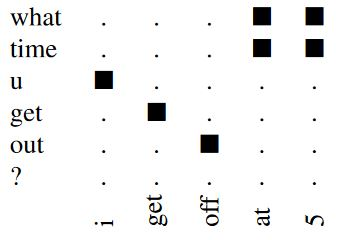
\includegraphics[width=0.7\linewidth]{pictures/generate.jpg}}
	\caption{Example for a generated response \cite{b14}.}
	\label{generate}
\end{figure}
\\Figure \ref{generate} shows a good example for the creation of a response, based on the explained model. For every word from the user (left) the most fitting word, due to the trained model, got selected (bottom). The black squares are showing the connections.\\
\\
One possible problem for a given sentence is, that the model generates almost the same sentence as a response. This can happen, because identical word pairs are frequently observed together \cite{b14}. These similarities need to be filtered out.\\
A more complex challenge is the word alignment. In some instances there is not a 1-1 correspondence between words/phrases in the input sentence and words/phrases in the output sentence \cite{b6}. This problem is not yet sufficiently solved \cite{b14}. A possibility is, to use additional statistical measurements like significance, to remove pairs of input-output phrases, that do not align \cite{b14}.

\subsection{Knowledge Base}\label{sec::kb}
The Knowledge Base is the central point of intelligence for a Chatbot. It can be seen as a collection of information about the specific use case, that the bot is applied for \cite{b15}. So if a Chatbot is used, to provide general informations about a company, the Knowledge Base holds all the necessary data about that. Then, when a question is referring to details from the company, the Chatbot uses the information from the Knowledge Base and formulates a response, based on the Response Generation component.\\
The most general Knowledge Base, which can get used for both types of Chatbots, is an external system. This could be a database, where the Chatbot automatically fetches information, when needed. Also an additional data Source like Google is possible, which provides the bot with intelligence (e.g. a dog is an animal) \cite{b6}. Whenever simple information is needed, the Chatbot could send a web-request, to fetch information from Google.\\
There are several more ways to generate a Knowledge Base and most of them are based on the type of Chatbot.
\\
\subsubsection{Rule-based Chatbot}
For a rule-based Chatbot it is necessary, to formulate patterns out of the given information. It is totally plausible, to generate a Knowledge Base manually and write the patterns by hand, in particular when the use case is quite easy. In other instances the amount of data is so high or the use case is too general, so this is no option. Therefore the patterns need to be generated automatically.\\
\\
There are many Sources of information, that can be used for this task. One basic approach is, to derive patterns out of a set of questions and answers (QA-set), which are available on almost any website as Frequently Asked Questions (FAQ) \cite{b16}. So if the domain is the point of interest, many informations can be gathered right there. The hardest task is, to formulate correct patterns out of the questions from the dataset. Reference \cite{b16} proposes an approach, where filler-words that have no or low semantic meaning, are filtered out.
\begin{figure}[htbp]
	\centerline{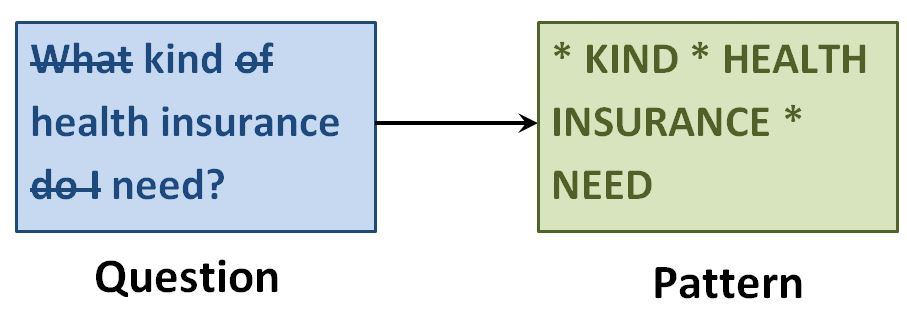
\includegraphics[width=1\linewidth]{pictures/knowledge.jpg}}
	\caption{Example for a generated pattern.}
	\label{knowledge}
\end{figure}
\\This is seen in figure \ref{knowledge}, where a question got transformed to a pattern. The filler-words (in the example: \textit{'what', 'of', 'do'} and \textit{'I'}) can be determined through calculation on a given text corpora, since they are often the most frequent words overall \cite{b16}. Additionally, they can be detected, when sentences on the same semantic topic get compared with each other, because only the relevant words are most likely the same \cite{b16}. The appropriate answers from the QA-set can often be used without any manipulation. Only in some instances the formulations need to be a bit more general, which has to be changed manually.\\
\\
Obviously, this is just one example, there are many more Sources, which can be used, to generate a Knowledge Base for a rule-based Chatbot, for example, glossaries or lexicons. The important step is always, to generate patterns out of the given data, which reflects the potential input from the user. In the discussed example it was possible, to automate the generation of patterns, based on the structure the QA-set already was. This is a really rare case, because most of the data is more unstructured, so the algorithm needs to know the different ways, a human can formulate a question, which is an extremely complex procedure. That means in a lot of cases, the patterns need to be written manual, which can be very time consuming and is one of the big disadvantages from rule-based Chatbots.
\\
\subsubsection{AI Chatbots}
Generally, the Knowledge Base for an AI Chatbots is the used training-data for the Machine Learning models, used in the Response Generation and NLP-part of the bot. So data is needed for the Intent and Entity approach, that relates to the specified topic, so the NLP-system can identify Intents and Entities around that. Furthermore, appropriate answers for all those Intents are necessary in the Response Generation. When a generative approach is used (chapter \ref{sec::gm}), the Machine Learning model needs also training-data, which contain all necessary informations about the specific topic.\\
\\
There are obviously a lot of ways, to gather training-data. Firstly, there are many existing dialogue corpora about different topics, which are already annotated by humans and can be used as training-data. Reference \cite{b15} shows an approach, to extract information out of online forums. This is possible, thanks to theme-related discussion pages, where different topics are handled. Therefore, pages about specific topics can be filtered out. Also, the general style of a user who has a question or problem and relating answers or solutions from others, helps to get data in the typical question-answer-form. However, the goal is, to have valid request-reply-pairs from the forum, which can be used as training-data. \\
But there are also some problems: replies are often too short, full of mistakes and can be unrelated to the request. Also, not every reply refers to the request but to other replies \cite{b15}. These problems need to be considered and overcome.
\begin{figure}[htbp]
	\centerline{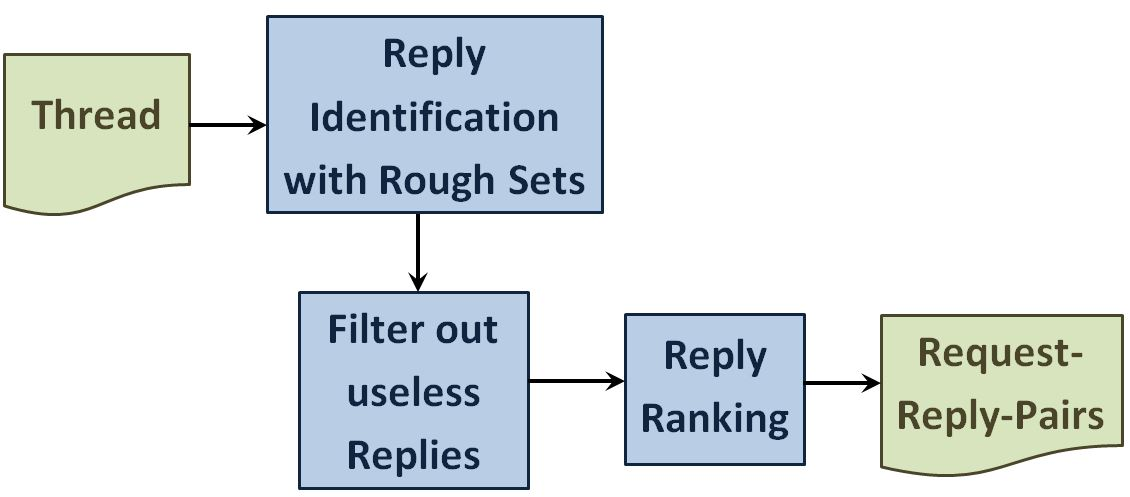
\includegraphics[width=1\linewidth]{pictures/ki_knowledge.jpg}}
	\caption{Steps to extract valid response-reply-pairs (based on \cite{b6}).}
	\label{kiknow}
\end{figure}
\\Figure \ref{kiknow} summarises the whole process, to find valid request-reply-pairs out of a forum thread. For every thread there are multiple pairs, depending on the amount of valid replies. The first target is, to identify the useful replies. Therefore, a Machine Learning technique called 'Rough Set' is used, which enables, to discover structural relationship within noisy data. This allows, to filter out replies, that are useless or refer to a different topic \cite{b15}. For this technique a model is set up, which ranks the replies on predefined features. The most important ones are \cite{b15}: 
\begin{itemize}
	\item Is  the  reply  posted  by  the  tread  starter?
	\item Does the reply quote the request or other messages?
	\item Does the reply use any of the predefined feature words?
	\item The number of words.
\end{itemize} 
In the next step the best rated replies get filtered out, based on bad language, the usage of 'my' and forum specific terms, since these replies are most often irrelevant or too noisy \cite{b15}. As a final step the replies are ranked, based on the rating from the Machine Learning model. The best rated request-reply-pairs can be used as the Knowledge Base and to train the Chatbot.\\
\\
Again, this is just one example, which allows to create a Knowledge Base. There are different possibilities to mine data for a Chatbot. It is just important, to get the data into a form, that has the typical question-answer-form.

\subsection{Dialogue Management}\label{sec:dial}
The final part from the Chatbot system takes care, to find communication strategies and language tricks, so the conversation with the bot is easier and in some cases even more human \cite{b6}. Also, the goal of these methods is, to deal with errors from the Chatbot itself and the user. General speaking, this is a wide-ranging topic. That is why, this chapter focuses mainly on error handling and tricks, that make the communication with the bot more easier and fluent. However, these strategies need to be considered, before developing the Response Generation, since they are influencing, how it operates. All the methods can be used for both a rule-based and AI Chatbot.
\\
\subsubsection{Error Handling}
The first discussed strategies tries to prevent errors. There are multiple approaches for this. One of them tries to make sure, that the user understands, what the bot can do. In particular the first system prompt should be a detailed description, on what the system has to offer and how the user can interact with it \cite{b17}. Example:\\
\textbf{System:} \textit{Hello, this is a bot, which helps you, to find PC-parts. If you search a specific PC part, please be sure to enter the name of it, a price-range and the brand name. If you want any additional information to a part, always write the name of the part in your question.}\\
If the dialogue has a complicated structure, the bot should repeat all commitments, that the user already made \cite{b17}. Example:\\
\textbf{User:} \textit{I want to buy a graphic card, that costs 500€.}\\
\textbf{System:} \textit{The graphic card should cost 500€, any other specifications?}\\
Another strategy is to ensure, that the bot is not inviting the user, to take initiative, which can lead to non-related questions. Most of the time the bot should lead the user to the expected behaviour and point them to the correct input \cite{b17}. Example:\\
\textbf{System:} \textit{In which PC-part are you interested?}\\
\textbf{User:} \textit{A graphic card.}\\
\textbf{System:} \textit{Which price range do you want?}\\
\textbf{User:} \textit{500€-600€} ...\\
Additionally, it is important, to point out Entity names such as locations or names, because they are often the most relevant informations and should always be recognised. Therefore, the system should specifically ask the user, to enter those Entities. Example:\\
\textbf{System:} \textit{Before you tell me, which PC-part you want, in which country do you live?}\\
\textbf{User:} \textit{In Germany.} ...\\
These are just a few strategies to prevent errors, but in some instances an error is happening nonetheless. Whenever this happens, it is important, to detect the error at an early stage and bring back the conversation to the correct path \cite{b17}. Therefore, a history of the conversation can be helpful, which allows the user and the system, to be aware of the context and detecting the specific point of miscommunication, to revert it \cite{b17}. Finally, what can be really helpful in these situations, is humour \cite{b17}. Although, it does not improve the quality of the dialogue or solves any problems, it can help, to relax the user, so no stress comes up.
\\
\subsubsection{Language Tricks}
There are some linguistic tricks that can be used, to improve the outcome of a conversation and make the bot act more human. This technique can help Chatbots, which have a medium chance, to generate correct responses, so the performance gets improved overall. In reference \cite{b18} some strategies are discussed:
\begin{itemize}
	\item \textbf{React to single-word sentence:} When the user types meaningless single words or letters like \textit{'d'}, \textit{'dd'} or \textit{'test'}, the bot can answer something like: \textit{'Talk to me in complete sentences, please.'}, to deal with it.
	\item \textbf{Switch topics:} The bot can propose a different topic to talk about. The requirement is, that the bot has knowledge on the proposed topic. This can also be used, to guide the user to another topic, if the bot has little or no knowledge on the current subject of discussion. The bot always needs to handle this discrete, so the the topic switch is not too abrupt and the conversations still feels natural.
	\item \textbf{End topics with an open question:} Rather then leading the conversation in a dead end, the Chatbot tries to reply back with a question, for example: \textit{'Sorry, i don't know. Do you want to see any PC-parts?'}.
	\item \textbf{Elicit more information:} The Chatbot can ask the user for more information on the current topic (\textit{'Could you tell me more about that?'}). This can get used by the Chatbot, to collect more knowledge on the specific topic. In some instances the bot could even ask the user, to define a unknown word and save this definition for later usage.
\end{itemize}
\ \\
Some other strategies aim, to make the Chatbot appear more human. Therefore, Small Talk can be really helpful, since human revert to neutral talk, when they are faced with task-specific situations \cite{b19}. Another more questionable feature has to do with failures. Often flawless communication may indicate, that the Chatbot is not human \cite{b19}, but making mistakes, is often stressful for the user. So the target is, to include some inconsistencies in the course of conversation, which are not too annoying for the user.\\
A different technique aims, to develop a personality for the bot. This starts with giving the bot a name (ELIZA, ALICE) and making him act like a specific character. ELIZA \cite{b1}, which is one of the first Chatbots,  has the personality of a psychologist, for example \cite{b19}. This can also include, that the Chatbot expresses emotions, for example, when the bot does not like spiders and the topic switches towards that, the bot replies repulsive. Or if the user types something insulting, the bot can react offended and even resentful later.

\section{Frameworks (both)}\label{sec:frameworks}
The last chapter was about the work methods of Chatbots. It is shown clearly, that the approaches are quite complicated, so in most of the cases it is pretty unrealistic, to build a Chatbot from ground up, since it is a complex and time consuming process. That is why there are several frameworks presented in this chapter, which help to develop and deploy a Chatbot.\\
For rule-based Chatbots the Artificial Intelligence Markup Language (AIML) is explained. Then the framework Rasa is presented, which allows to program AI Chatbots. The last framework is a commercial system called Dialogflow from Google, that also helps with creating an AI Chatbot.

\subsection{AIML (Fabio Aubele)}
AIML is a scripting language made for rule-based Chatbots. It is is a derivative of Extensible Mark-up Language (XML), which is based on the usage of different tags. Thanks to the simple structure of XML-files and thus AIML-files, it is really easy, to write patterns and create a naive bot. Therefore, an AIML-interpreter is needed, which is available for Java, Python, C++, NodeJS and more programming languages. The downloadable library-files include the interpreter and different functions, to set up a Chatbot instance in the program code. Also, it is possible, to configure many settings, which relate to the behaviour and properties of the Chatbot. In this section the basic functionality and important concepts of AIML are presented.\\
\\
Initially, any bot configuration is based on the following things \cite{b20}:
\begin{itemize}
	\item \textbf{AIML files:} Each bot has its own set of AIML files, which defines the personality of the bot. All necessary patterns and responses get written in these files. Normally, for every function or topic there is one file.
	\item \textbf{Learn file:} This is the central AIML file, where so-called brains are defined, which consist of multiple AIML-files. Each brain has a pattern, which needs to be entered first, to initiate the loading of the subordinated AIML-files.
	\item \textbf{Bot properties:} These are global values for a bot, such as a name for the Chatbot, logging or language settings.
\end{itemize}
Now the structure of an AIML file will be presented. In Code \ref{aiml} a simple AIML-file is shown.
\begin{lstlisting}[caption={Example of an AIML file (based on \cite{b20}).},label=aiml,lineskip=1pt]
<?xml version="1.0" encoding="UTF-8"?>

<aiml version="2.0">
<category>
  <pattern>HI *</pattern>
  <template>Hello world!</template>
</category>

<category>
  <pattern>What is a chatbot</pattern>
  <template>
    A Chatbot is a computer program, designed to
    respond to text inputs in natural language.
  </template>
</category>
</aiml>
\end{lstlisting}
In the first lines some XML and AIML properties are set, then the first AIML object, called Category is defined. These are the basic rules for matching an input from the user to an output from the bot. Each Category consists of a Pattern, which is the potential input and a Template, which is the answer from the Chatbot to the user.\\
The Pattern can include letters, numbers, spaces, and Wildcard symbols \cite{b21} but no special characters or punctuation, they are ignored in the user input. One Wildcard symbol already shown in Code \ref{aiml} is \textit{'*'}, this stands for one or more words in the input \cite{b20}. So thanks to the Wildcard the input: \textit{'Hi my good friend.'} or \textit{'Hi bot.'}, would also be recognized, but only \textit{'Hi'} would not be detected. Another Wildcard symbol is \textit{'\textasciicircum'}, which expresses zero or more words \cite{b20}. So if this Wildcard would be used in Code \ref{aiml}, the input \textit{'Hi'} would now also be recognized. The interpreter always prioritises exact matches over a Wildcard match.\\
\\
In order to ensure different necessary functionalities, multiple tags and functions are introduced in AIML. Only the most important ones will be presented here\footnote{For a full list of all tags and functions, see \href{https://www.pandorabots.com/docs/aiml-reference/}{https://www.pandorabots.com/docs/aiml-reference/}}. The first one is the \textbf{topic-tag}, which encloses different Categories. When a topic is set, only the Categories inside the topic are matched against the input from the user. This helps, when Pattern are quite equal, but related to different content. Based on the state of the conversation, it is possible, to change the topics inside the Categories \cite{b20}. In Code \ref{aiml_topic} an example is shown.
\begin{lstlisting}[caption={Example for the topic-tag (based on \cite{b20}).},label=aiml_topic,lineskip=1pt]
<category>
  <pattern>LET US TALK ABOUT *</pattern>
  <template>
    OK, I like <set name="topic"><star/></set>
  </template>
</category>

<topic name="coffee">

<category>
  <pattern>I DRINK IT PLAIN</pattern>
  <template>
    I prefer mine with cream and sugar
  </template>
</category>

</topic>
\end{lstlisting}
In the first Category the user sets a potential topic with the Wildcard symbol (referred as <star/> in the Template). If the topic was \textit{'coffee'}, the second Category, which is enclosed in the topic \textit{'coffee'}, can get triggered with the right input. Now, different topics can be created, for example, if the Chatbot should also react to the topic \textit{'tea'}, it just needs to be introduced in the AIML file. Then it is even possible, to write the exact same Pattern \textit{'I DRINK IT PLAIN'} with a different Template. In summary, Categories wrapped in the topic-tag only trigger, if the user ask for this topic in advance.\\
\\
Another pretty common tag is \textbf{<random>}. Therefore, the user defines multiple replies in a list inside the Template tag\cite{b20}. The interpreter chooses one reply randomly. This is useful for common Patterns, so the bot answers diversified.\\
Also, pretty important is the \textbf{srai-tag}, which refers to rules for recursive reduction \cite{b20}. This can be useful for three different applications. The first one is reducing complex grammatical forms to simpler ones \cite{b21}. Another application is the divide and conquer approach, that splits an input into two or more sub-parts and combines the responses for each \cite{b21}. The last one deals with synonyms by mapping different forms of the same Pattern to the same reply \cite{b21}. In Code \ref{aiml_srai} an example for the usage of srai is shown. 
\begin{lstlisting}[caption={Example for the srai-tag (based on \cite{b21}).},label=aiml_srai,lineskip=1pt]
<category>
  <pattern>HALO</pattern>
  <template>
    <srai>Hello</srai>
  </template>
</category>
\end{lstlisting}
In this case srai is defining \textit{'HALO'} as a synonym for \textit{'Hello'} to deal with misspelling. \textit{'Hello'} has to be a different Pattern, that already exists, \\
Another needed function are \textbf{'Predicates'}, which are local variables, to store string values from the user input. These Predicates can get used inside Categories as a reference to important values, that got named earlier. The AIML standard does not specify, where the Predicates are defined, most often they get introduced directly in the Categories.\\
\\
AIML is also known, for being used, to create the Chatbot ALICE (Artificial Linguistic Internet Computer Entity), which was first implemented by Wallace from 1995 onwards and won the annual Loebner Prize Competition\footnote{The Loebner Prize is an annual competition, that honors programs, which are considered the most human-like by the judges.} in Artificial Intelligence three times. This is also the reason AIML rose in popularity. Furthermore, ALICE is also available as an open Source program.

\subsection{Rasa (Joshua Hörmann)}
Rasa is an open-Source framework for building AI Chatbots in Python. It is used by thousands of developers worldwide, thanks to the focus on consistent API's with different back-end implementations \cite{b22}. The framework is separated into Rasa NLU (Natural Language Understanding) and Rasa Core. Another part is Rasa X, which is a tool that helps the Chatbot, to learn from real conversations and improve it further. In this paper Rasa NLU and Core is discussed.
\\
\subsubsection{Rasa NLU}
Rasa NLU takes care of any task, related to NLP and uses the Intent and Entity approach, discussed in chapter \ref{sec:inform}. The aim is, to find out the Intent and Entities of any utterance from a possible user. In Code \ref{rasanlu} an example is shown for an utterance and the consequential output.
\begin{lstlisting}[caption={Potential output of Rasa NLU for a given utterance (based on \cite{b22}).}, label=rasanlu, lineskip=1pt, language=json, morekeywords={intent, entities, part, price}]
Utterance: "I am looking for a graphic card, which 
costs 500€."
Output:
"intent": "search_part",
  "entities":
    "part" : "graphic_card",
    "price" : "500"
\end{lstlisting}
In order to achieve this behaviour, a number of NLP and Machine Learning libraries are combined in an API \cite{b22}. At the start of every project a Machine Learning model needs to be set-up and trained with data. It is recommended, to structure the data in a markdown-format, since this is also human readable \cite{b22}. Code \ref{rasanlu2} shows, how the training-data need to be structured correctly. 
\begin{lstlisting}[caption={Trainings data for Rasa NLU (based on \cite{b22}).}, label=rasanlu2, lineskip=1pt, language=json,
morekeywords={intent, entities, part, price, graphic card, 500}]
## intent:search_part
- I want something for my pc
- I am looking for a [graphic card](part) which 
costs [500](price)€
- I need a [graphic card](part)

## intent:greet
- hey
- hello
\end{lstlisting}
First the overall Intent has to be mentioned, then a list of the potential utterances are named. It is important, that the Entities are in the form [entity](entity name), so it is possible for the Machine Learning model, to extract them correctly. Additionally, it is feasible, to define synonyms for Entities. \\
\\
In comparison to the rule-based approach, not every possible utterance for the specific Intent needs to be named. If enough example are given, the model can also assign utterances to their correct Intents, which are not exactly named in the listing, but are similar to the other examples. Therefore, some of the words and the sentence structure need to be equal, so it is still necessary, to specify enough examples. The same does not really apply for Entities, since Rasa needs at least one example for every potential value, to extract the Entity correctly. Only if the Entities are build equally or appear always at the same position of the sentence, it is feasible to extract them automatically with enough training sentences. In order to find the best amount of examples, for automatically extracting Intents and Entities, some testing is necessary.\\
The output from the model for an utterance is already shown in Code \ref{rasanlu}, the only thing, which gets added, is a Confidence-Score from the Machine Learning model between zero and one, that expresses, how certain the given Intent and the found Entity is correct.\\
Rasa NLU allows to choose and fine-tune the Machine Learning model, so it fits on different datasets. Presenting all the different models and configurations is beyond the scope of this work\footnote{Detailed information are listed on \href{https://rasa.com/docs/rasa/nlu/choosing-a-pipeline/}{https://rasa.com/docs/rasa/nlu/choosing-a-pipeline/}}.
\\
\subsubsection{Rasa Core}
The second part of Rasa takes care of all tasks related to Dialogue Management and Response Generation. The main format, to train the Rasa dialogue management models, are called Stories. These Stories are a representation of a conversation between a user and the Chatbot \cite{b22}. In order to understand the structure of these Stories, some terms have to be defined:\\
\\
\textbf{Actions:} These are the responses from the bot to the user. There are mainly two different types of Actions: Utterance Actions which send a specific predefined textual message to the user and Custom Actions which run additional code in form of a function, to perform an arbitrary action, like turning on the lights through an API call, fetch something from a database or anything else \cite{b22}.\\
\textbf{Slots:} The Slots are the memory of the bot, which act as a key-value store. They can be used, to store any kind of information, the user provided aswell as information gathered about the outside world (by a database query for example) \cite{b22}. It is possible, to make the Slots influence the dialogue progression (just continue if the Slot is set). \\
\textbf{Policies:} The Policy is the Machine Learning model, that decides, which Actions get executed for the given Intent and Entities. They get trained with the written Stories, which describe the flow of the conversation. There are different Policies, to choose from, each of them differ in their used technology and approach on how they decide, which response to take. In most of them the important factors are: what was the last Action, what are the Intent and Entities in the most recent user message and which Slots are currently set. \cite{b23}\\
\textbf{Domain:} The Domain defines the universe, in which the Chatbot operates. It specifies the Intents, Entities, Slots, and Actions the bot should know about \cite{b22}. It is basically an overview of all functions from the bot.\\
\\
Like already said, the Stories are the most important part from Rasa Core. In Code \ref{rasacore} an example is showcased.
\begin{lstlisting}[caption={Example for a Story in Rasa Core (based on \cite{b23}).}, label=rasacore, lineskip=1pt, language=json,
morekeywords={intent, search_part, inform, greet}]
## story_07715946
* greet("name":"Fabio")
  - slot{"name": "Fabio"}
  - utter_ask_howcanhelp
* search_part
  - utter_on_it
  - utter_ask_part
* inform{"part":"graphic_card"}
  - utter_ask_price
* inform{"price":"500"}
  - action_info_part
\end{lstlisting}
The first line gives the Story a name, which is mainly needed for debug purposes \cite{b23}. Then the first message from the user is shown in the form \textit{'intent\{"entity1": "value", "entity2": "value"\}'}. After that the responses from the Chatbot are listed with the starting symbol \textit{'-'}. The first one defines a Slot for the given Entity \textit{'name'}. Then a Utterance Action is defined. This structure continues in the example, only at the end the response \textit{'action\_info\_part'} is a Custom Action, which performs the search for the pc part.\\
For all Utterance Actions the textual responses need to be defined. This is done in the Domain under Templates. In Code \ref{rasacore2} an example is presented.
\begin{lstlisting}[caption={Example for templates in Rasa Core (based on \cite{b22}).}, label=rasacore2, lineskip=1pt, language=json,
morekeywords={templates}]
templates:
utter_ask_howcanhelp:
- text: "Hi, how can i help you?"
- text: "Hello, is there anything i can do?"
\end{lstlisting}
At first the Utterance Action is named, then two possible responses are specified. Thus, the Chatbot will randomly pick one of them \cite{b22}. It is also feasible, to use Slots in the responses. Custom Actions do not need a textual response in the domain, since additional Python code takes care of them.\\
\\
Like already discussed for Rasa NLU, the Machine Learning approach in Rasa Core allows some freedom, in deciding, which Action to take next. That means not every potential outcome in the dialogue flow, needs to be written as a Story. If enough examples are given, the system can guess the responses correctly. There is always some testing necessary, to find the best amount of Stories.

\subsection{Google Dialogflow (Joshua Hörmann)}
Google Dialogflow is a commercial framework for creating conversational assistants. It allows, to build both voice- and text-based interfaces, but the focus in this work lies on textual bots. Thanks to the Machine Learning approaches from Google and complex NLP techniques, the API is really powerful. The building platform is web-based and can be reached with every internet browser. The focus lies on an easy-to-use interface and the opportunity, to integrate the Chatbot in other services \cite{b24}. Dialogflow also offers a free version with limited functionalities. In this section the basic process of creating a bot and the main functions will be presented. Also it is shown, how it is possible, to integrate the bot into other services.\\
\\
Dialogflow names the Chatbot an Agent. At the start an Agent needs to be created, there are different configurations, which can be changed like language, logging settings and more. There is also the opportunity, to start with a pre-built agent, that already is able to hold small talk with the user or has other basics for conversation on a specific topic \cite{b24}.\\
The terminology in Dialogflow is almost the same like already discussed. The basic conversation is structured in Intents, which describe the input from the user and responses, that express the answers from the Agent. Furthermore, so-called Actions are used for executing logic. In figure \ref{google} a form is shown, that is used to create a new Intent.  
\begin{figure}[htbp]
	\centerline{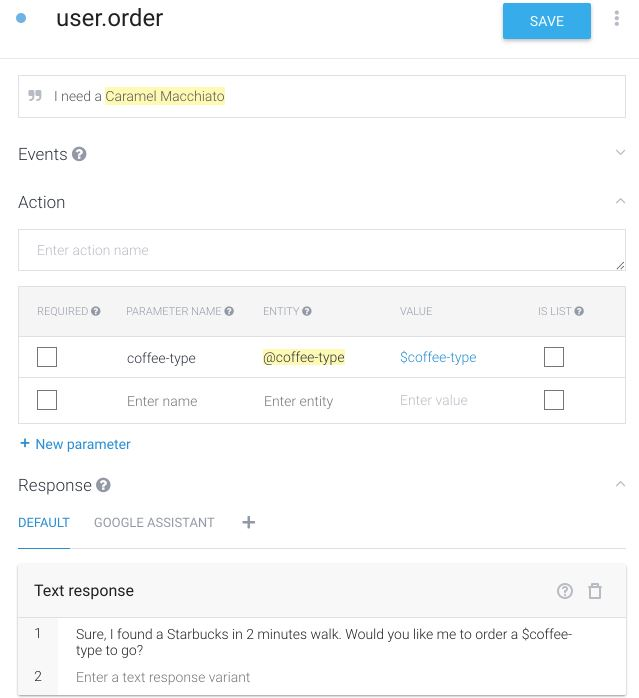
\includegraphics[width=1\linewidth]{pictures/google.jpg}}
	\caption{Form to create a new Intent in Dialogflow \cite{b24}.}
	\label{google}
\end{figure}
\\The example is about a coffee order and the form confirms the focus on an easy-to-use interface. It is also feasible, to select default Intents for standard phrases in a conversation like a greeting or goodbye. Every Intent describes, what the user says as an textual representation. Not every possible phrase is defined here, since Dialogflow's built-in Machine Learning tool expands the list with other similar phrases \cite{b24}. Each Intent can have different parameter, also called Entities. Each Entity has a type, which describes the parameter (\textit{'coffee-type'} in figure \ref{google}) and potential values (Caramel Macchiato, Cappuccino, etc.) \cite{b24}. There is also the possibility, to create synonyms for each value. The Entities are created in a different form, in figure \ref{google} only the parameter must be entered. At last there is a textual response from the agent. It is also feasible to use the Entities here. \\
\\
Another needed feature are Actions, which are executing logic. This could be a call to an external API or a web-hook, that needs to be executed \cite{b24}. In the example in figure \ref{google} it would be the actual ordering process of the coffee. Since Dialogflow provides the extracted Entities from the user expression, they can be used as parameter for the Action. There is even a process, that helps, to gather all the information from the user, if some parameters are missing to fulfil an Action \cite{b24}.\\
A not yet discussed term from Dialogflow is Context, which is needed, to handle user expressions, so Dialogflow understands, what the user is referring to \cite{b25}. It can be seen as the general topic, the user and the bot is talking about. Each Intent has an Input Context and an Output Context \cite{b25}, this allows to enable topic switches. The Input Context specifies the state of conversation, in which the Intent is handled. In contrast, the Output Context is the state, in which the conversation is, when the Intent was handled successfully and a response was output \cite{b25}.\\
\\
A different feature allows to define additional training-data for the Machine Learning model, to improve its performance. Since Dialogflow logs all the conversations of the agent, it is feasible, to use this data directly, to train the model \cite{b24}. It is just necessary, to upload the log, then all user messages and the assigned Intents are listed. It is possible, to correct certain user messages, Intents and Entities or even delete some entries, if they do not fit as training-data \cite{b24}.\\
Google's Dialogflow allows to directly test the created agent in the web interface. On the right side of the website, there is always a simulator. This is a useful tool, to test, that the agent behaves as expected. Also, it is possible, to integrate the Chatbot seamlessly on many popular conversation platforms like Facebook, Skype, Twitter, Telegram or others with just a button press \cite{b24}. Another powerful feature is, the possibility to integrate the bot directly on a website. Dialogflow generates HTML-code, which can get copied and pasted on the appropriate website. Evens a dummy website is supplied, where the integration can be tested.

\section{Deployment (Joshua Hörmann)}\label{sec:deployment}
After presenting several frameworks we get to the question how to deploy the chatbot and what you need to keep in mind there. 
Hence this chapter starts with the various deployment options. After that the key points which should be considered are named. 

\subsection{Hosting Options}
There are several options for hosting the boot. Figure \ref{SaaSvsOP} shows the two most common Software as a Service (SaaS) and On Premises and the development of their share of the enterprise application market. On Premises was the common concept until approx. 2010\cite{b26}, afterwards on premise continuously lost proportions to SaaS. Below the deploy options local, Software as a Service, On Premises, and On-Premises in Foreign Data Center are described.

\begin{figure}[htbp]
	\centerline{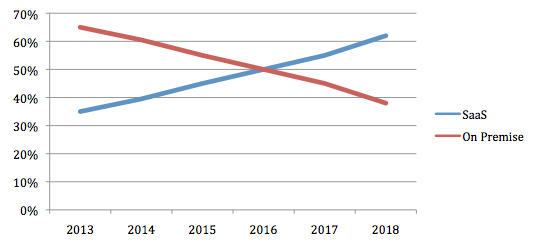
\includegraphics[width=1\linewidth]{pictures/SaaS-vsOn-premise.png}}
	\caption{Development of On Premise and SaaS Enterprise Applications from 2014 to 2018 \cite{b27}.}
	\label{SaaSvsOP}
\end{figure}

\subsubsection{local}
Local deployment means that all services run on the same physical machine. The server is running on the same hardware as the user that communicates with the bot. The use-case for this form of deployment is quite small, because this would only meet the requirements if the bot should only have one user at a time and the chatbot shouldn't have a connection to the internet. Furthermore every change to the bot has to be done on that one particular computer. So if one wants to update the bot, he has to go to the computer and for the whole time of the update the computer is blocked. With a server-client architecture one can still run the old instance of the bot, update another one and then switch from the old to the new one. In addition one don't have to go to the computer and it won't be blocked for the user. Because of the above mentioned restrictions local deployment isn't considered a reasonable way to deploy the software. Moreover most of the nowadays used Chatbots are used on websites, what favours a distributed system. But local deployment it is good for testing purposes and to get in touch with chatbots.

\subsubsection{On-Premises}
Another form of deployment is called on-premises, also known as software as a product. On-Premises means that the chatbot runs on-site where he is used. The bot has to be installed and must be maintained from the company that uses it, not from the company that builds the bot. Therefore costs for hardware, maintenance and operation must be taken into account.\cite{b26} If the used bot isn't open Source, there are additional costs for the license, that must be observed. A good example for On-Premise aside chatbots is Microsoft Office. You pay for it one time and install it on your own computer. You are responsible for it and if something happens to your computer all data and the whole settings are lost, if you didn't made a backup.

\subsubsection{Cloud-Computing}
The opposite of On-Premises is, Cloud-Computing or Software as a Service (short SaaS). As the name intends, here the chatbot is a service. The customer just rents a package, which includes software, hardware, maintenance and the operation of the bot. Hence the chatbot is running on a server in the data center of the vendor, or a data center which is partnered with them. The contract for SaaS solutions is normally time-limited. \cite{b26} There is obviously no additional cost for the chatbot if is included in the rented package. The SaaS counterpart for Microsoft Office is Office 365, here you can use all the office programs like word or excel inside the browser of your choice. With normal settings it saves your preferences and it is linked with Microsoft's cloud solution OneDrive. So if you use this together you can access your programs and data from every device that is linked to the internet.  
\subsubsection{On-Premises in Foreign Data Center}
There is also the option to run the chatbot on-premise but in a foreign data center, so not the vendor's data center. But the big problem here is that this combines the disadvantages of On-Premise and Cloud-Computing. Thus there are two contracts with two different vendors and if the operator of the data center doesn't cover the installation and maintenance of the software. The customer has to do all that on his own. But there are some of the advantages aswell, the automated backup in a data center for example.
\subsection{Key Points}
This section describes various Key Points to consider when choosing how to deploy. For every point it also gives a evaluation.
\subsubsection{Framework Choice}
The choices of the framework has a big impact on the deployment. Because some chatbots are restricted to a certain deploy method.
\begin{description}
\item[On-Premises]\hfill \\
The above mentioned Open Source Rasa framework can be used On-Premises \cite{b22}, but Google Dialogflow can´t.
\item[Cloud-Computing]\hfill \\ 
There is also a enterprise version of Rasa that uses a paid subscription and cloud computing. \cite{b22} Google Dialogflow only can be used hosted by Google with a paid subscription. \cite{b28}
\item[On-Premises in Foreign Data Center]\hfill \\
All On-Premises chatbots can be installed and run from a foreign data center aswell.
\end{description}

\subsubsection{Costs}
Money is always a factor and it also has to be considered by the choice of the deploy method. This of course only applies if costs are incurred. If it's just for test purposes, the most frameworks got trial versions. 
\begin{description}
\item[On-Premises]\hfill \\
Initially very high costs for the purchase of the hardware and perhaps the software, but afterwards only the operating costs, like electricity and maintenance costs. \cite{b29} 
\item[Cloud-Computing]\hfill \\ 
Only monthly charges due to the subscription. All costs for server, infrastructure and maintenance is covered by the vendor.\cite{b29} 
\item[On-Premises in Foreign Data Center]\hfill \\
Initially costs for the software, if it's not open Source and additionally the monthly charges for the server in the data center.
\end{description}

\subsubsection{Availability}
Another key point is the availability of the chatbot for the user. This depends on the usage of the chatbot, if the he is implemented into a website it should be available around the clock. If he only is accessible on selected PCs inside a company the availability isn't a big problem. The time the server is available is called uptime. 
\begin{description}
\item[On-Premises]\hfill \\
The availability of a On-Premises chatbot depends on various factors: the on-site internet connection, the used server room facilities and more. For example if a Uninterruptible Power Supply (UPS) is installed to prevent shutdowns due to power grid fluctuations. 
\item[Cloud-Computing]\hfill \\ 
A data center is equipped with everything to get a high availability. Most data centers guarantee a uptime of 99 \%. \cite{b30}
\item[On-Premises in Foreign Data Center]\hfill \\
Because the chatbot is hosted in a data center, there is also a availability of 99\%.
\end{description}

\subsubsection{Data Control}
The control over the data, that builds the basis of the chatbot. And of course the data that is generated by the bot.
\begin{description}
\item[On-Premises]\hfill \\
This is a big advantage of On-Premises solutions, because there the company (or person) that utilize the chatbot has the full control over the bot and the data. Because it is all stored on-site the protection and the direct control are guaranteed. \cite{b29}
\item[Cloud-Computing]\hfill \\ 
With Cloud-Computing the data has to be transferred to the data center and all communication between the user and the chatbot is stored there aswell. Hence it is a higher risk, to use Cloud-Computing. But it has to be mentioned that there are several data centers with certifications towards data safety.
\item[On-Premises in Foreign Data Center]\hfill \\
Again the data has to be transferred to the data center, so the same applies as for cloud computing.
\end{description}

\subsubsection{Technical Knowledge}
Another key feature to mention here is the technical knowledge. For the different deployment methods one needs several technical skills.
\begin{description}
\item[On-Premises]\hfill \\
With self-hosting all the technical knowledge is required to update the infrastructure and the application. \cite{b29}
\item[Cloud-Computing]\hfill \\ 
Because the company that hosts the chatbot handles all technical aspects, for Cloud-Computing is just little knowledge required. \cite{b29}
\item[On-Premises in Foreign Data Center]\hfill \\
Here the need of technical knowledges depends on the contract with the data center, but normally the data center takes over the update of the infrastructure. So the knowledge to update the chatbot is required.
\end{description}

\subsubsection{Scalability}
The scalability defines how easy it is to expand the chatbot. That is needed if the chatbot collects data over time, or if the amount of users, which use the bot, is strongly increasing.
\begin{description}
\item[On-Premises]\hfill \\
At On-Premises the upgrade has to be made physical on the on-site server. \cite{b29} If more data space is needed, a hard drive upgrade has to be done or if the amount of users increases the CPU and/or the RAM has to be upgraded.
\item[Cloud-Computing]\hfill \\ 
A upgrade of a Cloud-Computing chatbot is quite easy, because either a upgrade to a better (more powerfull) package is available or the booked package scales with the requirements.
\item[On-Premises in Foreign Data Center]\hfill \\
The same applies here as for cloud computing.
\end{description}

\subsubsection{Backup}
The last key point to mention here is the Backup. A good backup of the chatbot and the data behind it is crucial, to be prepared for a system crash or a virus attack.
\begin{description}
\item[On-Premises]\hfill \\
The backup at Open-Premises has to be done manually through a tape drive or a Network Attached Storage.
\item[Cloud-Computing]\hfill \\ 
Normally a backup of the whole server is included in the package that you rent at the data center.
\item[On-Premises in Foreign Data Center]\hfill \\
Once again applies the same as for cloud computing, because the chatbot and the data are stored on a server inside the data center.
\end{description}


\section{Framework Comparison (Joshua Hörmann)}\label{sec:comparison}
After all the informations are gathered and the functionalities are clarified, a comparison of the above mentioned chatbot frameworks AIML, Rasa and Google Dialogflow can be established. Therefore the criterias are listed and after that the comparison will be done. Finally the Pros and Cons of the three Frameworks AIML, Rasa and Google Dialogflow are listed.
\subsection{Criterias}
The following criteria are mostly taken from the paper "Comparison of Various Chatbot Frameworks" by Vatsal Shah and Dr. Seema Shah. \cite{b31} The framworks will be compared regarding:
\begin{itemize}
\item \textbf{Speech Processing} : Can the framework process speech aswell?
\item \textbf{Prebuild Entities} : Has the framework prebbuild entities included?
\item \textbf{Prebuild  Intents} : Has the framework prebuild intentents included?
\item \textbf{supported programming languages} : Which programming languages are supported?
\item \textbf{Online Integration} : Are there any thrid party integrations available?
\item \textbf{Machine learning} : Does the framework use machine learning?
\item \textbf{License} : How is the framework licensed? Is it opensource?
\item \textbf{Languages} : Which Languages are supported?
\end{itemize}

\subsection{Comparison}
Below is the table that compares the chatbot frameworks based on the given criteria.
\begin{tabularx}{0.45\textwidth}{|p{0.125\textwidth}|X|X|X|X}
\hline
& AIML & Rasa & Dialogflow \\
\hline
Speech Processing & No & No & Yes\\
\hline
Pre-build Entities & No & No & Yes\\
\hline
Pre-build Intents & No & No & Yes\\
\hline
supported programming languages & Python, Node.js, PHP, Ruby & Java, Ruby, Python, C++, C\#, Pascal & Java, C\#, Go, Node.js, PHP, Python, Ruby\\
\hline
Online Integration Yes & Yes & Yes &\\
\hline
Machine learning & No & Yes & Yes\\
\hline
License & Opensource & Opensource and enterprise bersion & Free standard edition and enterprise editions\\
\hline
Languages & any Language & any Language & all common languages\\
\hline
\end{tabularx}

\subsection{Pros \& Cons}

\subsubsection{AIML}
\paragraph{Pros}
\begin{quote}
\begin{itemize}
\item easy to learn
\item simplicity of the system
\item good readable for humans and computer (through XML)
\end{itemize}
\end{quote}
\paragraph{Cons}
\begin{quote}
\begin{itemize}
\item elaborate input data creation for extension
\item must be updated periodically
\item no intelligence, just pattern matching
\end{itemize}
\end{quote}

\subsubsection{Rasa}
\paragraph{Pros}
\begin{quote}
\begin{itemize}
\item Open Source
\item High adaptability
\item fully offline usable
\end{itemize}
\end{quote}
\paragraph{Cons}
\begin{quote}
\begin{itemize}
\item Time-consuming training
\item can only deployed on-premises
\item training of the bot on your hardware
\end{itemize}
\end{quote}

\subsubsection{Google Dialogflow}
\paragraph{Pros}
\begin{quote}
\begin{itemize}
\item easy support for small-talk
\item training on google servers
\item clear code editor 
\item many Integrations for Messenger
\end{itemize}
\end{quote}
\paragraph{Cons}
\begin{quote}
\begin{itemize}
\item fee-based version for professionals
\item dependent on google
\item can only be deployed with Cloud Computing
\end{itemize}
\end{quote}

\section{Conclusion (both)}
The target of this work was to define and explain the main work methods of a Chatbot and present some frameworks, which can help, to create a bot. Additionally the most common deployment methods were introduced. The first presented work method is NLP, which helps, to parse the input from the user into a form the computer understands. The structured input gets used by the Response Generation, which defines a response with the potential help of a Knowledge Base, where information can get fetched from. The last part is the Dialogue Management, which can provide strategies, that influence the generation of a response. Then three frameworks are presented. AIML enables to create rule-based Chatbots with a scripting language, that is based on XML. The second framework Rasa helps to create AI Chatbots and is split into two parts. Rasa NLU allows to extract Intent and Entities out of the input from a user and Rasa Core takes care of the Dialogue Management and Response Generation. The last framework was Google Dialogflow, which is the only commercial one and also used to create AI Chatbots. The focus lies on an easy-to-use interfaces and the possibility, to integrate the Chatbot on other conversation platforms.\\
\\
It is important to point out, that rule-based Chatbots almost always have the big disadvantage, that it is time consuming, to create all the patterns for a specific use case. On the other hand it is possible, to create a naive Chatbot really fast and without much effort. By contrast AI-Chatbots need training-data, but a lot of frameworks offer techniques or tools, which help generating data easily. However, the selection process for the right Machine Learning approach can be quite complex, since they rely on correct configuration and application.\\
The most important part of any Chatbot is the Response Generation, which needs to define the correct output for the utterance the user made. This part should always get the most focus, when developing a Chatbot. In the frameworks this part was defined through different structures, which represented a conversation and had statements for the Chatbot and the user. \\
Also important is the decision which method is used for deployment. Hence the most used ones local, On-Premises and Cloud-Computing (SaaS) are introduced. Local is only a valid option for testing or in some exceptions. On-Premises and Cloud-Computing both got their advantages and disadvantage, but the final decision depends on the used framework and the use-case. 
In the future this work can get complemented with more example for the defined work methods. Also it is feasible to present even more frameworks or showcase the already presented ones on a practical example and compare their advantages/disadvantages with each other.


\begin{thebibliography}{00}
\bibitem{b1} Jospeh Weizenbaum, ''Computer Power and Human Reason: From Judgment to Calculation'', Freeman and Company, United States, 1976, pp. 2, 3, 6, 182, 189.
\bibitem{b2} Ian Cairns, ''Speed up customer service with quick replies \& welcome messages'', Source: \href{https://blog.twitter.com/marketing/en_us/topics/product-news/2016/speed-up-customer-service-with-quick-replies-welcome-messages.html}{https://blog.twitter.com/marketing/en\_us/topics/product-news/2016/speed-up-customer-service-with-quick-replies-welcome-messages.html}, Twitter Marketing, United States, November 2016, Accessed: 24.10.2019.
\bibitem{b3} Drift, ''The 2018 State of Chatbots Report'', 2018, United States, pp. 16.
\bibitem{b4} M.Dahiya, ''A Tool of Conversation: Chatbot'', Maharaja Surajmal Institute, Dept. of Computer Science, India, April 2017, Vol. 5, Issue 5.
\bibitem{b5} Bayan AbuShawar, Eric Atwell, ''ALICE Chatbot: Trials and Outputs'', Arab Open University, IT department, Amman, Jordan, University of Leeds, School of Computing, Leeds, UK, 2015, pp. 625-632.
\bibitem{b6} Jack Cahn, ''CHATBOT: Architecture, Design, \& Development'', University of Pennsylvania, Department of Computer and Information Science, United States, April 2017.
\bibitem{b7} Mahipal Jadeja, Neelanshi Varia, ''Perspectives for Evaluating Conversational AI'', Dhirubhai Ambani Institute of Information and Communication Technology, India, September 2017.
\bibitem{b8} Kumar Shridhar, ''Rule based bots vs AI bots'', Source: \href{https://medium.com/botsupply/rule-based-bots-vs-ai-bots-b60cdb786ffa}{https://medium.com/botsupply/rule-based-bots-vs-ai-bots-b60cdb786ffa}, Medium, May 2017, Accessed: 31.10.2019.
\bibitem{b9} haptik, ''Understanding Conversational AI – What, Where \& How You Can Use Bots'', Source: \href{https://haptik.ai/blog/conversational-ai-bots-business-meaning/}{https://haptik.ai/blog/conversational-ai-bots-business-meaning/}, Accessed: 31.10.2019.
\bibitem{b10} Barbara Rychalska, Helena Głabska, Anna Wróblewska, ''Multi-intent Hierarchical Natural Language Understanding for Chatbots'', Faculty  of  Mathematics  and  Computer  Science,  Warsaw  University  of  Technology, Poland, 2018.
\bibitem{b11} Cyril Joe Baby, Faizan Ayyub Khan, Swathi J. N., ''Home Automation using IoT and a Chatbot using Natural Language Processing'', School of Electronics Engineering, School of Computer Science and Engineering, VIT University, India, 2017.
\bibitem{b12} Pavel Král, Christophe Cerisara, ''Dialogue Act Recognition Approaches'', University of West Bohemia, Czech Republic, LORIA UMR, France, November 2012.
\bibitem{b13} Zhao Yan, et. al., ''DocChat: An Information Retrieval Approach for Chatbot Engines Using Unstructured Documents'', State Key Laboratory of Software Development Environment, Beihang University, China, 2016.
\bibitem{b14} Alan Ritter, Colin Cherry, William B, ''Data-Driven Response Generation in Social Media'', Computer Sci. \& Eng.University of Washington, National Research Council Canada Dolan, Microsoft Research Redmond.
\bibitem{b15} Yu Wu, Gongxiao Wang, Weisheng Li, Zhijun Li, ''Automatic Chatbot Knowledge Acquisition from Online Forum via Rough Set and Ensemble Learning'',  Institute  of  Artificial Intelligence, Chongqing University of Posts and Telecommunications, China, 2008.
\bibitem{b16} Giovanni De Gasperis, ''Building an AIML Chatter Bot Knowledge-Base Starting from a FAQ and a Glossary'', Dipartimento Ingegneria Elettrica e dell’Informazione, Università degli Studi dell’Aquila, Italia, 2010.
\bibitem{b17} Andreea I. Niculescu, Rafael E. Banchs, ''Strategies to cope with errors in human-machine spoken interactions: using chatbots as back-off mechanism for task-oriented dialogues'', Institute for Infocomm Research, Singapore.
\bibitem{b18} Zhou Yu, et. al., ''Strategy and Policy Learning for Non-Task-Oriented Conversational Systems'', School of Computer Science, Carnegie Mellon University, United States, 2016.
\bibitem{b19} Maria Joao Pereira, Luísa Coheur, ''Just.Chat - a platform for processing information to be used in chatbots'', Instituto Superior T ́ecnico, Taguspark, Portugal, May 2013.
\bibitem{b20} Author unknown, ''AIML Docs'', Source: \href{http://www.aiml.foundation/doc.html}{http://www.aiml.foundation/doc.html}, June 2018, Accessed: 12.11.2019.
\bibitem{b21} Bayan Abu Shawar, Eric Atwell, ''Chatbots: Are they Really Useful?'', LDV Forum, Germany, issue 22.
\bibitem{b22} Author unknown, ''Rasa Docs'', Source: \href{https://rasa.com/docs/rasa/}{https://rasa.com/docs/rasa/}, 2019, Accessed: 14.11.2019.
\bibitem{b23} Tom Bocklisch, et. al., ''Rasa: Open Source Language Understanding and Dialogue Management'', Rasa, NIPS 2017 Conversational AI workshop, 2017.
\bibitem{b24} Google, ''Dialogflow Concepts'', Source: \href{https://cloud.google.com/dialogflow/docs/concepts}{https://cloud.google.com/dialogflow/docs/concepts}, 2019, Accessed: 15.11.2019.
\bibitem{b25} Srini Janarthanam, ''Hands-On Chatbots and Conversational UI Development'', Packt, United Kingdom, 2017, pp. 110-140.
\bibitem{b26}  Florian Karlstetter, "Was ist On-Premises?", 2017, Source: \href{https://www.cloudcomputing-insider.de/was-ist-on-premises-a-623402/}{https://www.cloudcomputing-insider.de/was-ist-on-premises-a-623402/}, Accessed: 01.02.2020
\bibitem{b27} C. Dover "IDC Worldwide SaaS Enterprise Applications 2014-2018 Forecast and 2013 Vendor Shares" 2017
\bibitem{b28} Stefan Luber, Nico Litzel, "Was ist Dialogflow?", Source: \href{https://www.bigdata-insider.de/was-ist-dialogflow-a-788455/}{https://www.bigdata-insider.de/was-ist-dialogflow-a-788455/}, 2019, Accessed: 30.01.2020.
\bibitem{b29} Michael Sweeney, "The Difference Between SaaS Applications and On-Premises", Source: \href{https://clearcode.cc/blog/saas-applications-vs-on-premises/}{https://clearcode.cc/blog/saas-applications-vs-on-premises/}, Accessed: 30.01.2020
\bibitem{b30} Reza Madjidi, "SaaS (Software as a Service) oder On premise? Eine Frage der Installation.", Source: \href{https://www.unatrix.com/de/blog/saas-oder-on-premise/}{https://www.unatrix.com/de/blog/saas-oder-on-premise/}, 2015, Accessed: 30.01.2020
\bibitem{b31} Vatsal Shah, Dr.Seema Shah, "A Comparison of Various Chatbot Frameworks", CIKITUSI Journal for Multi disciplinary Research Volume 6 Issue 1, 2019
\end{thebibliography}

\end{document}
